\section{Simulation Analysis}
\label{sec:simulation}

\subsection{Operating point Analysis (for t<0 and $v_s(t) = 0$)}

Ngspice was used to perform an operating point analysis for t<0 (obtaining table #) and by setting $v_s = 0$ and replacing the capacitor with a voltage sorce $V_x = V_6 - V_8$, the voltage and current values, present in tables below, were obtained.

\begin{table}[!h]
	\centering
	\begin{tabular}{|l|r|}
		\hline    
		{\bf Name} & {\bf Value [mA]} \\ \hline
		§R1 & 1.04309563061e+03 \\ \hline
§R2 & 2.01744623407e+03 \\ \hline
§R3 & 3.13691375104e+03 \\ \hline
§R4 & 4.15429988186e+03 \\ \hline
§R5 & 3.07915362723e+03 \\ \hline
§R6 & 2.02592738504e+03 \\ \hline
§R7 & 1.04226655522e+03 \\ \hline
§H1 & 8.25247516035e+03 \\ \hline
£G1 & 7.31630468385e-03 \\ \hline
Va & 5.23936486299e+00 \\ \hline
@Id & 1.03899051042e-03 \\ \hline


	\end{tabular}
	\caption{Constants provided by Python. A variable preceded by @ is of type {\em current}
		and expressed in Ampere;a variable preceded by § is of type {\it resistence} and expressed in
		Ohms;a variable preceded by £ is of type {\it conductance} and expressed in
		Siemens; other variables are of type {\it voltage} and expressed in
		Volt.}
	\label{tab:op}
\end{table}



\begin{table}[!h]
	\centering
	\begin{tabular}{|l|r|}
		\hline    
		{\bf Name} & {\bf Value [mA]} \\ \hline
		§R1 & 1.04309563061e+03 \\ \hline
§R2 & 2.01744623407e+03 \\ \hline
§R3 & 3.13691375104e+03 \\ \hline
§R4 & 4.15429988186e+03 \\ \hline
§R5 & 3.07915362723e+03 \\ \hline
§R6 & 2.02592738504e+03 \\ \hline
§R7 & 1.04226655522e+03 \\ \hline
§H1 & 8.25247516035e+03 \\ \hline
£G1 & 7.31630468385e-03 \\ \hline
Va & 5.23936486299e+00 \\ \hline
@Id & 1.03899051042e-03 \\ \hline


	\end{tabular}
	\caption{Constants provided by Python. A variable preceded by @ is of type {\em current}
		and expressed in Ampere;a variable preceded by § is of type {\it resistence} and expressed in
		Ohms;a variable preceded by £ is of type {\it conductance} and expressed in
		Siemens; other variables are of type {\it voltage} and expressed in
		Volt.}
	\label{tab:op}
\end{table}


\subsection{Transient Analysis - Natural Response}

The first step in order to compute the natural response of $v_6$ is to set $v_s(t) = 0$ and set initial conditions so that $v_6$ and $v_s$ have the same values obtained in table 10, which ensures that in the start of the transient analysis the capacitor is fully charged. The graphic in figure 11 was obtained by executing a transient analysis, with t ranging from o to 20 ms.

By analyzing the graphic we can see a quick drop in voltage from just a little above 8 ms to 0, which is due to the fact that the capacitor is just discharging and since there are no independent voltage sources, there is no voltage being provided to $v_6$.

\begin{figure}[h] \centering
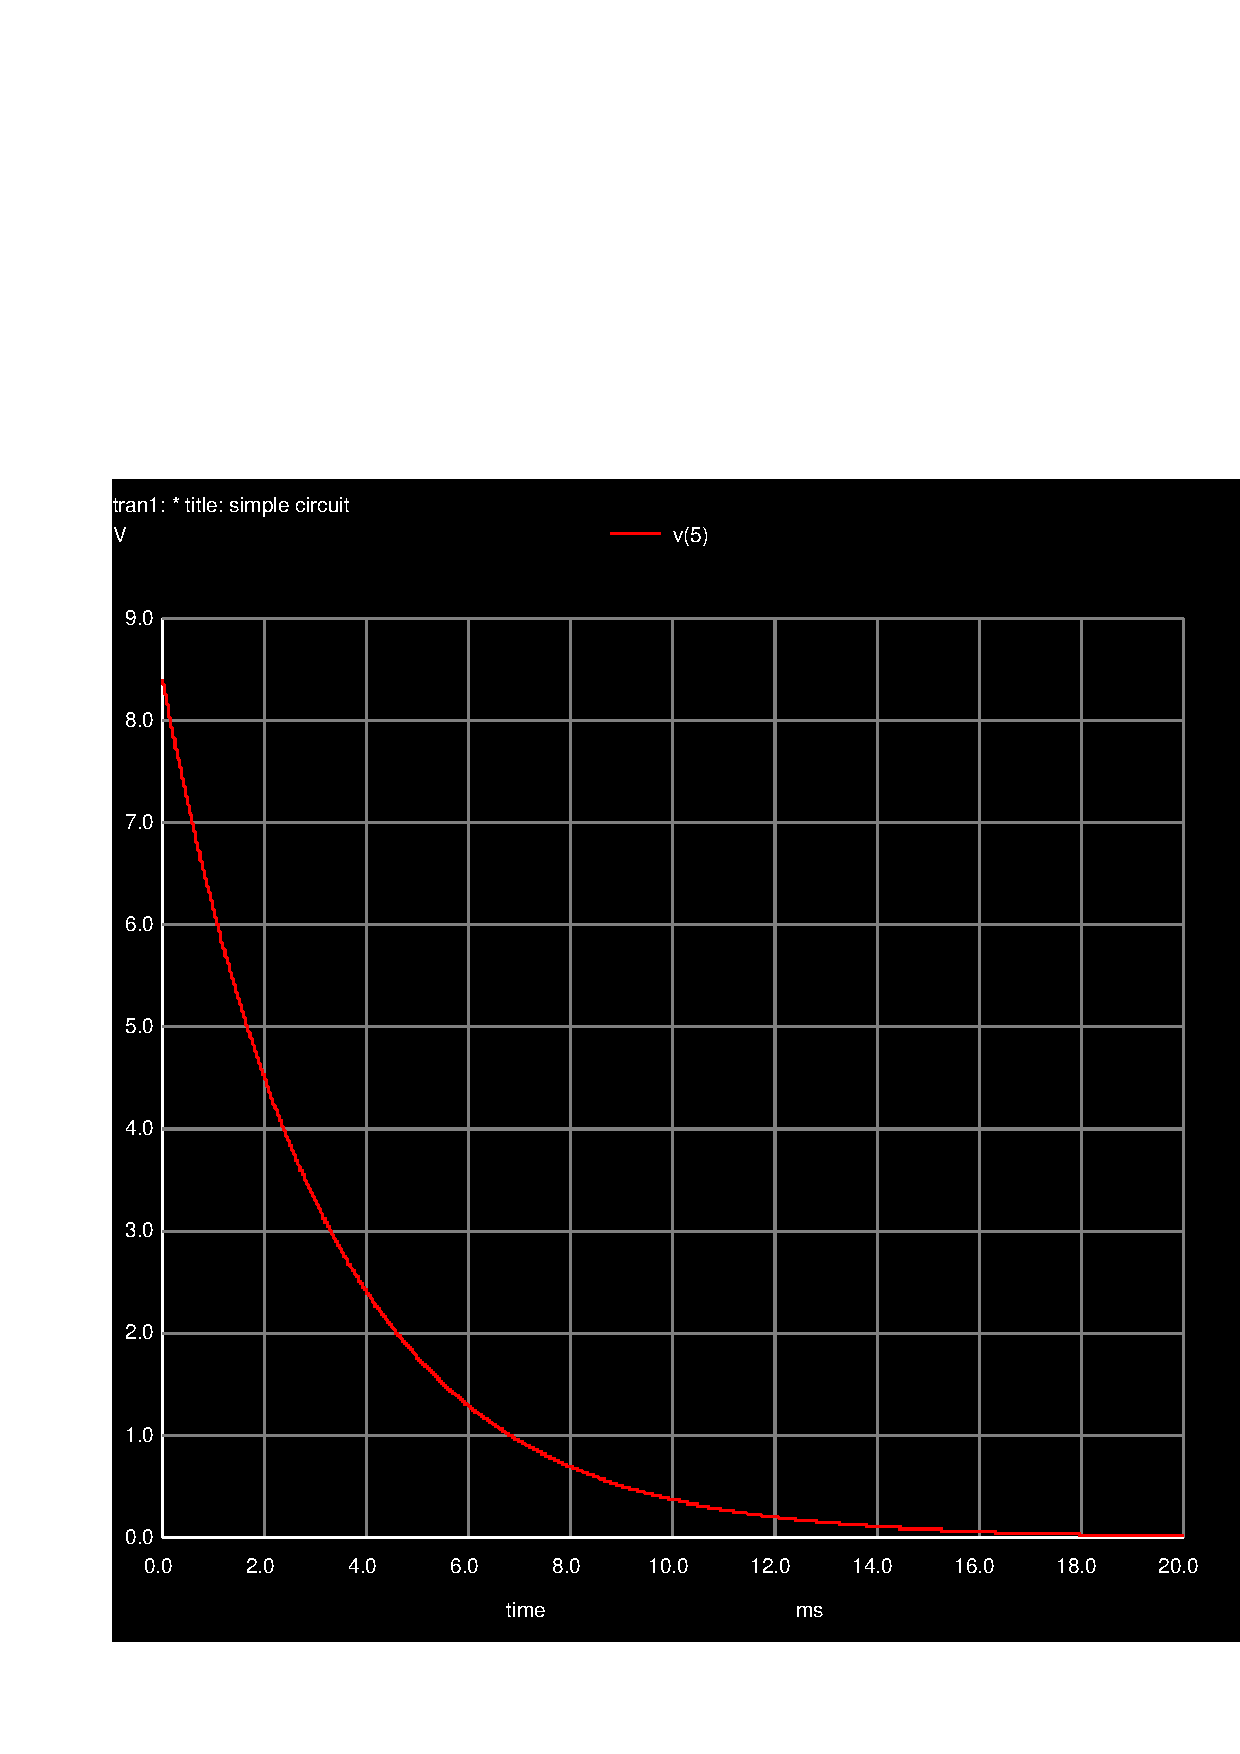
\includegraphics[width=0.6\linewidth]{trans.pdf}
\caption{.}
\label{fig:rc1}
\end{figure}


\subsection{Transient Analysis - total Response}

Taking in consideration that $v_s(t) = \sin(2\pi ft)$ and f = 1000Hz, the total response can be obtained by performing a transient analysis and the figure 12 can be obtained by plotting $v_s(t)$ and $v_6(t)$. 

\begin{figure}[h] \centering
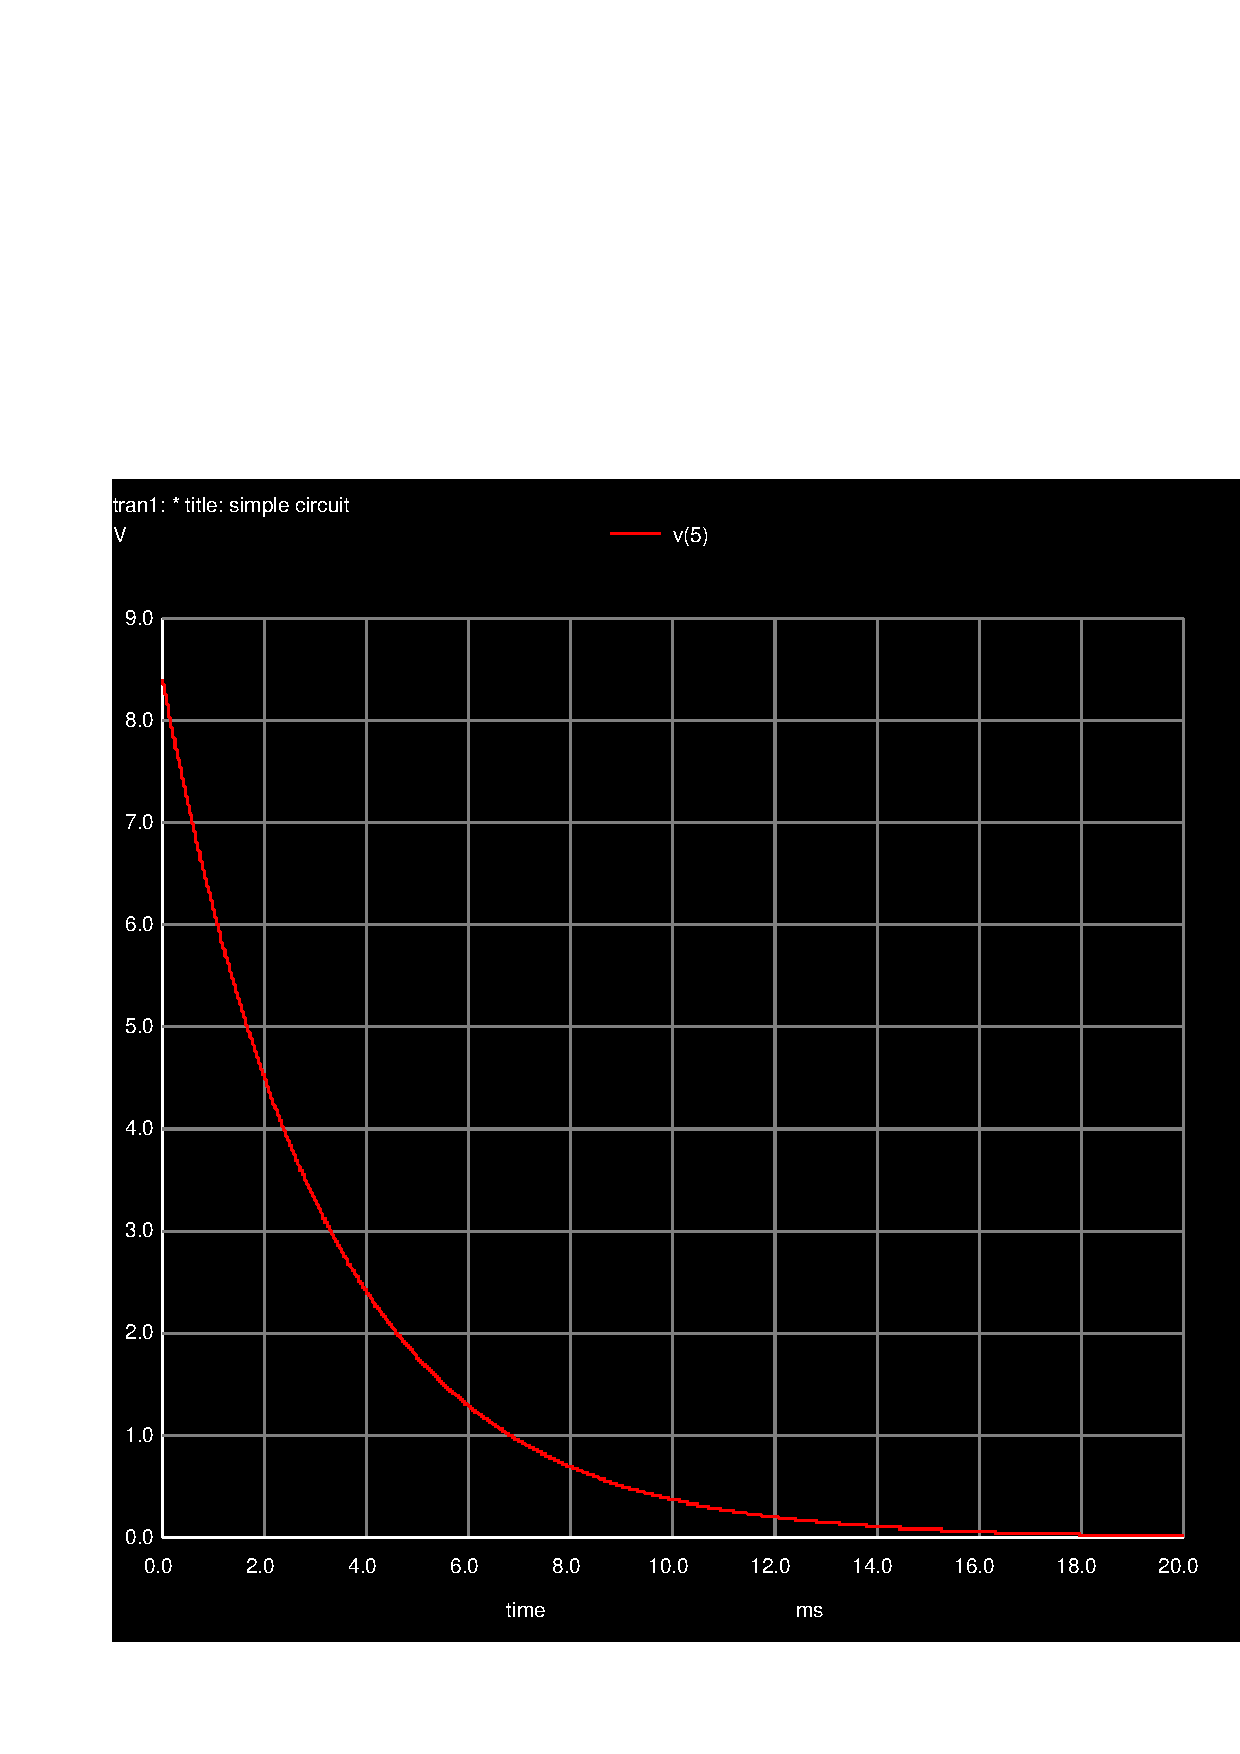
\includegraphics[width=0.6\linewidth]{trans.pdf}
\caption{.}
\label{fig:rc1}
\end{figure}


\subsection{Frequency Response}

By excuting a frequency sweep, throughout the length of the interval [0.1, 1000000], we are able to plot the magnitude and phase, which appear below respectively.
\begin{figure}[h] \centering
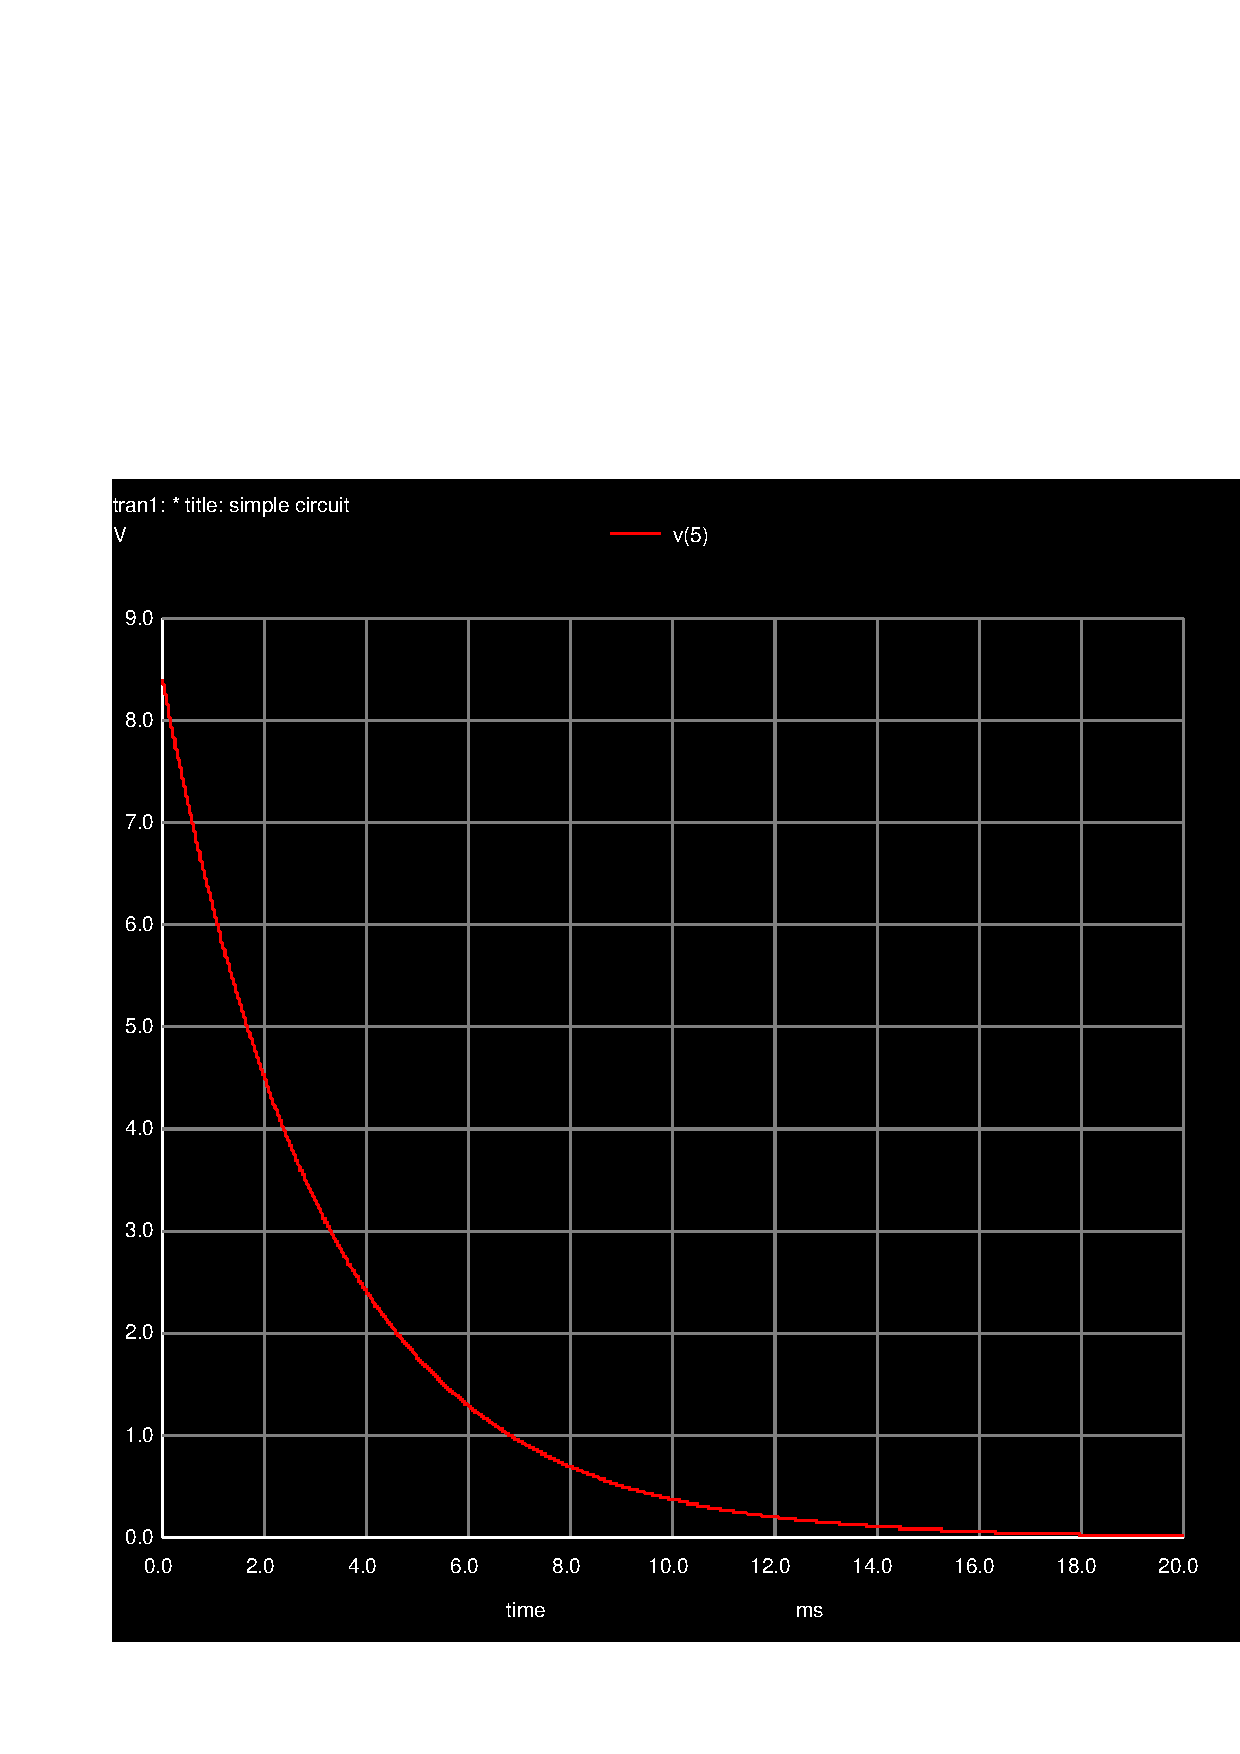
\includegraphics[width=0.6\linewidth]{trans.pdf}
\caption{.}
\label{fig:rc1}
\end{figure}



\begin{figure}[h] \centering
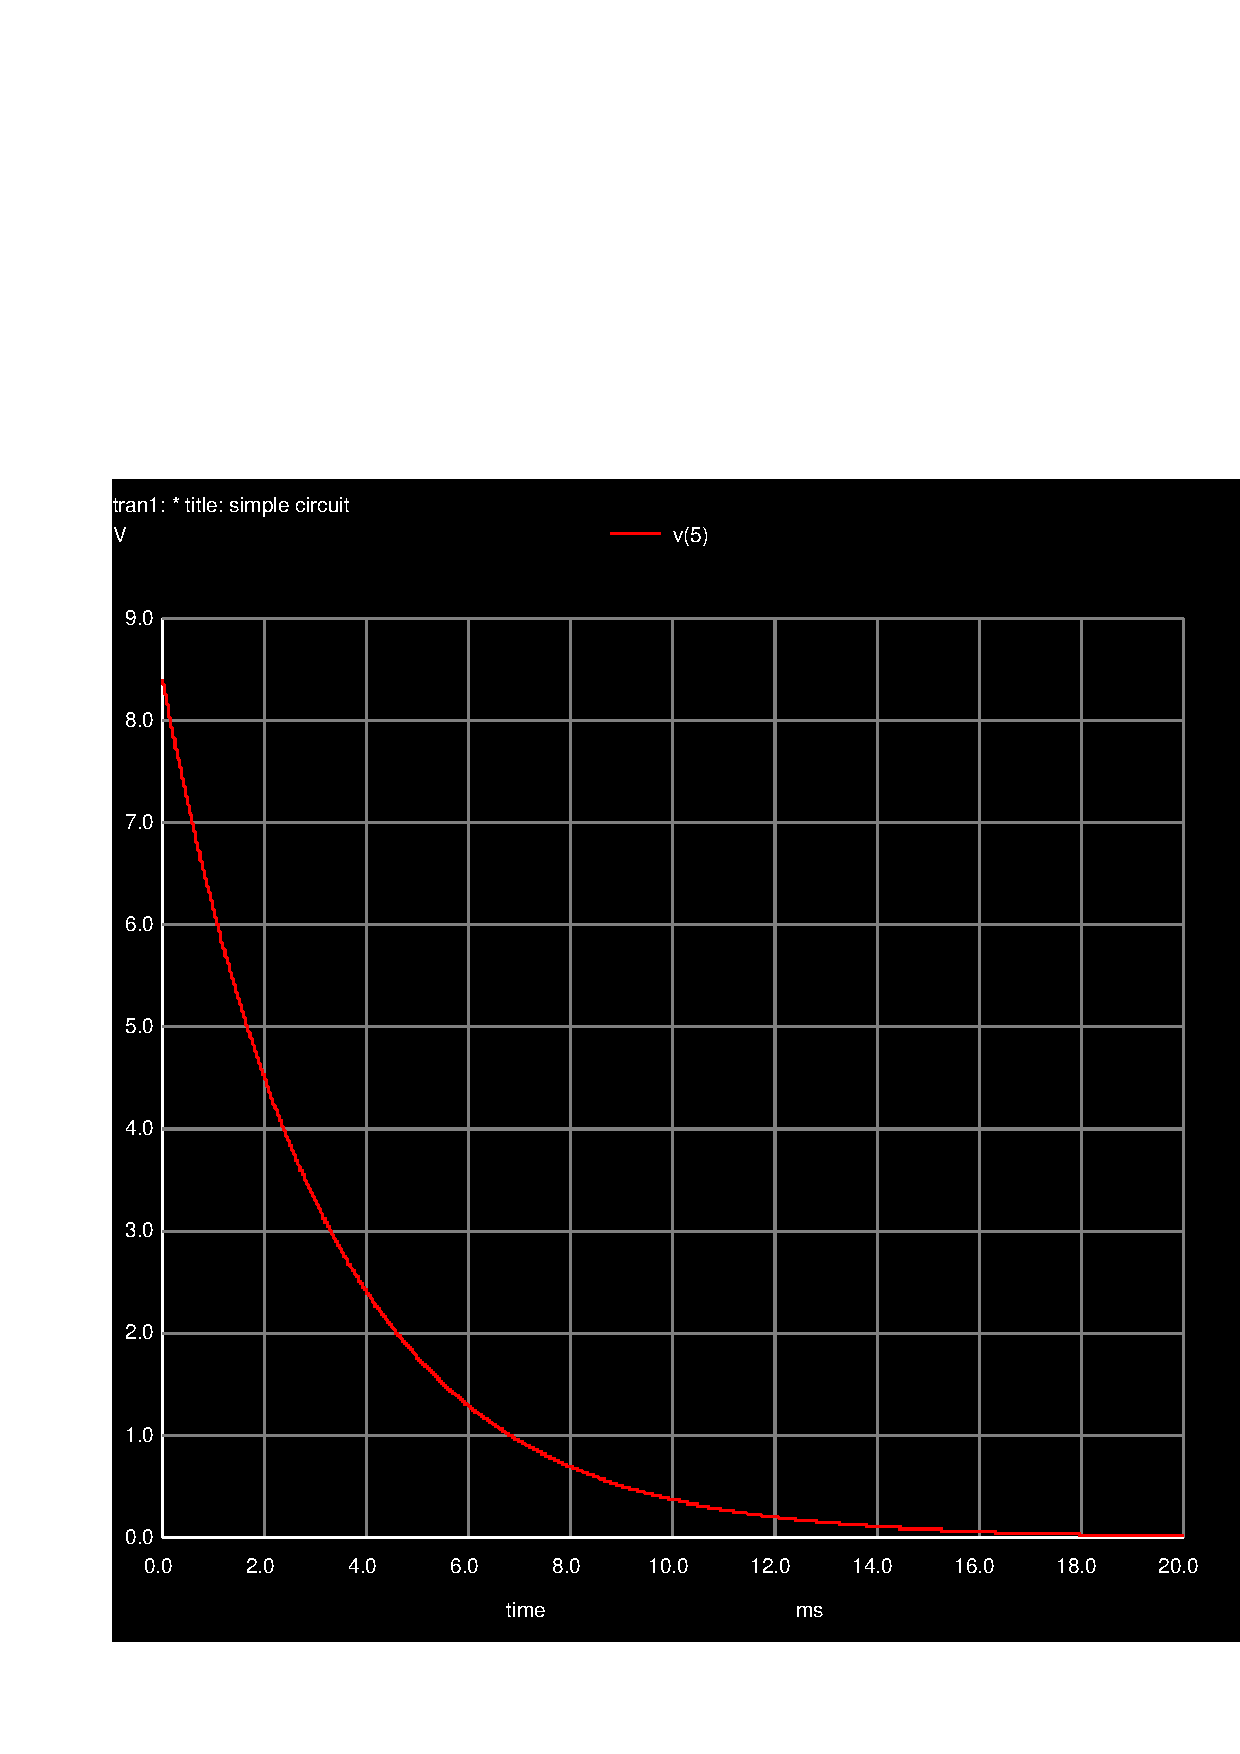
\includegraphics[width=0.6\linewidth]{trans.pdf}
\caption{.}
\label{fig:rc1}
\end{figure}

